\chapter{Πρωτόκολλα Αρχιτεκτονικής}
\label{chap:Protocols}

\section{Εισαγωγή}

Στο παρόν κεφάλαιο περιγράφονται τα πρωτόκολλα του συστήματος. Η βιβλιοθήκη 
έχει βασιστεί στο P-Grid και επομένως υλοποιείται ο αλγόριθμος exchange 
όπως έχει οριστεί στο \citep{Abererb}. Θα γίνει μια μικρή περιγραφή του. 
Στη συνέχεια αναλύεται διεξοδικά το πρωτόκολλο ανοχής λαθών που η ανάπτυξή 
του είναι και ένας από τους στόχους της διπλωματικής εργασίας.

\section{Πρωτόκολλο Exchange}

To P-Grid δίκτυο κατασκευάζεται μέσω των αλληλεπιδράσεων μεταξύ των peer. 
Ο τρόπος με τον οποίο ένα P-Grid δίκτυο κατασκευάζεται είναι μέσω του 
αλγορίθμου exchange. Στα σχήματα \ref{algo:ExchangePart1} και 
\ref{algo:ExchangePart2} παρουσιάζεται ο αλγόριθμος και ακολουθεί η 
ανάλυση του.

Αρχικά, κατά τα πρώτα στάδια εκκίνησης του δικτύου, οι peer είναι υπεύθυνοι 
για όλο τον χώρο κλειδιών. Δεν υπάρχουν κατατμήσεις και όλοι οι peer 
αντιστοιχούν στο ριζικό μονοπάτι του δέντρου. Ο αλγόριθμος exchange 
καθορίζει τον τρόπο με τον οποίο ο χώρος κλειδιών θα διασπαστεί σε 
περισσότερες εξειδικεύσεις. Κάθε μια από αυτές τίθεται υπό την ευθύνη 
ενός peer. Ο αλγόριθμος εκτελείται με την πρώτη ευκαιρία που δύο peer 
θα συναντηθούν.

Οι peer ελέγχονται πάνω στο μονοπάτι για το οποίο είναι υπεύθυνοι. 
Σε κάθε εκτέλεση του αλγορίθμου, οι δυο peer ανανεώνουν τους πίνακες 
δρομολόγησης τους. Αρχικά, ανταλλάσσουν τυχαία αναφορές προς peer για όλα 
τα επίπεδα του κοινού προθέματος.

\paragraph{Περίπτωση 1.} Η πρώτη περίπτωση του αλγορίθμου προκύπτει όταν 
αυτοί αντιστοιχούν στο ίδιο μονοπάτι, έστω $x$. Τότε και οι δύο peer 
εξειδικεύονται περαιτέρω προς αντίθετες κατευθύνσεις. Ο ένας θα αναλάβει 
το μονοπάτι $χ0$ και ο άλλος το συζυγές $χ1$. Κάθε peer προσθέτει τον άλλον 
στον πίνακα δρομολόγησης ως υπεύθυνο για το νέο επίπεδο που δημιουργήθηκε 
στο μονοπάτι.

\paragraph{Περιπτώσεις 2 και 3.}Η δεύτερη και η τρίτη περίπτωση είναι 
παρόμοιες. Το μονοπάτι του ενός peer είναι μικρότερο από αυτό του άλλου 
και μάλιστα είναι και πρόθεμα του. Στην περίπτωση αυτή, ο λιγότερο 
εξειδικευμένος peer προχωρά προς την αντίθετη κατεύθυνση. Αν παράδειγμα 
αυτός είχε το μονοπάτι $x$ και ο άλλος peer το $x1$, τότε ο πρώτος 
εξειδικεύεται προς το $x0$. Επίσης, ανανεώνονται και οι αναφορές στους 
πίνακες δρομολόγησης. Παρατηρούμε, πως αν ο peer $a1$ αντιστοιχεί το 
μικρότερο μονοπάτι, τότε κατά την εκτέλεση του αλγορίθμου αυτός θα είναι 
στην δεύτερη περίπτωση ενώ ο $a2$ στην τρίτη.

\paragraph{Περίπτωση 4.} Τέλος, έχουμε την περίπτωση όπου οι δυο peer 
μοιράζονται ένα κοινό πρόθεμα αλλά από εκεί και μετά έχουν ακολουθήσει 
διαφορετικού δρόμους στο δέντρο. Εδώ ο αλγόριθμος εκτελείται αναδρομικά. 
Οι peer $a1$ και $a2$ προωθούν αιτήσεις για εκτέλεση του αλγορίθμου στους 
peer που έχουν αποθηκευμένους στους πίνακες δρομολόγησης. Όταν 
το δίκτυο φτάσει στην τελική του μορφή, ο χώρος κλειδιών θα έχει διασπαστεί 
σε τόσα κομμάτια όσος και ο αριθμός των peer. Τότε θα προκύπτει συνεχώς η 
τέταρτη περίπτωση κατά την εκτέλεση του αλγορίθμου. Η σταθερά $recmax$ 
θέτει ένα άνω όριο στον αριθμό των αναδρομών που θα εκτελεστούν και είναι 
μια συνθήκη τερματισμού.

\begin{algorithm}
\caption{Αλγόριθμος Exchange, μέρος 1ο}
\label{algo:ExchangePart1}
\begin{algorithmic}[1]
    \Procedure{Exchange}{a1, a2, r} 
        \State commonpath = common\_prefix\_of(path(a1), path(a2));
        \State lc = length(commonpath);
        \If{(lc > 0)}
        \Comment{exchange references at the level where the paths agree}
            \State commonrefs = union(refs(lc, a1), refs(lc, a2));
            \State refs(lc, a1) = random\_select(refmax, commonrefs);
            \State refs(lc, a2) = random\_select(refmax, commonrefs);
            \State l1 = length(sub\_path(path(a1), lc + 1, length(path(a1))));
            \State l2 = length(sub\_path(path(a2), lc + 1, length(path(a2))));            
\newline \Comment{Case 1: if both remaining paths are empty introduce a new level}
            \If{(l1 = 0 $\And$ l2 = 0)}            
                \State path(a1) = append(path(a1), 0);
                \State path(a2) = append(path(a2), 1);
                \State refs(lc + 1, a1) = {a2};
                \State refs(lc + 1, a2) = {a1};
            \EndIf
\newline \Comment{Case 2: if one remaining path is empty split the shorter path}
            \If{(l1 = 0 $\And$ l2 > 0)}
                \State path(a1) = append(path(a1), $\neg$value(lc + 1, path(a2)));
                \State refs(lc + 1, a1) = {a2};
                \State refs(lc + 1, a2) = random\_select(refmax, union({a1}, refs(lc + 1, a2)));
            \EndIf
\algstore{ExchangeBreak}
\end{algorithmic}
\end{algorithm}

\begin{algorithm}[h]
\caption{Αλγόριθμος Exchange, μέρος 2ο}
\label{algo:ExchangePart2}
\begin{algorithmic}[1]
\algrestore{ExchangeBreak}
\item[] \Comment{Case 3: like case 2}
            \If{(l1 > 0 $\And$ l2 = 0)}
                \State path(a2) = append(path(a2), $\neg$value(lc + 1, path(a1)));
                \State refs(lc + 1, a2) = {a1};
                \State refs(lc + 1, a1) = random\_select(refmax, union({a2}, refs(lc + 1, a1)));
            \EndIf
\newline \Comment{Case 4: recursively perform exchange with referenced peers}
            \If{(l1 > 0 $\And$ l2 > 0 $\And$ r < recmax)}
                \State refs1 = refs(lc + 1, a1) $\setminus$ {a2};
                \State refs2 = refs(lc + 1, a2) $\setminus$ {a1};
                \For{r1 $\in$ refs1}
                    \If{online(peer(r1))}
                        \State exchange(a2, peer(r1), r + 1)
                    \EndIf
                \EndFor
                \For{r2 $\in$ refs2}
                    \If{online(peer(r2))}
                        \State exchange(a1, peer(r2), r + 1)
                    \EndIf
                \EndFor
            \EndIf
        \EndIf
  \EndProcedure
\end{algorithmic}
\end{algorithm}


\section{Πρωτόκολλο Ανοχής Λαθών (Fault-Tolerance)}
\label{sec:Fault}

\subsection{Γενικά}

Για να κατανοήσουμε τι είναι η ανοχή λαθών ας δούμε τα χαρακτηριστικά 
ενός αξιόπιστου συστήματος. 

\begin{description}
\item [Διαθεσιμότητα (Availability).] Αντιπροσωπεύει την ετοιμότητα του 
συστήματος. Συγκεκριμένα είναι η πιθανότητα το σύστημα να λειτουργεί 
σωστά σε κάποιες χρονικές στιγμές και να εκτελεί σωστά τη 
λειτουργικότητα που προσφέρει.
\item [Αξιοπιστία (Reliability).] Είναι η ικανότητα του συστήματος να 
λειτουργεί συνεχόμενα χωρίς αποτυχίες. Είναι η πιθανότητα να λειτουργεί 
σε ένα χρονικό διάστημα.
\item [Ασφάλεια (Safety).] Η κατάσταση όπου το σύστημα αποτυγχάνει 
προσωρινά χωρίς να συμβεί κάτι καταστροφικό.
\item [Δυνατότητα συντήρησης (Maintainability).] Η ευκολία με την οποία 
επιδιορθώνεται το σύστημα.
\end{description}

Η εκπλήρωση των παραπάνω χαρακτηριστικών επιτυγχάνεται με τη μείωση των 
αποτυχιών που συμβαίνουν στο σύστημα και την συνεχή παροχή των υπηρεσιών 
του για το οποίο έχει σχεδιαστεί. Αυτή είναι και η ουσία της έννοιας 
«ανοχή λαθών». Οι αποτυχίες χωρίζονται σε διάφορες κατηγορίες. Μπορεί να 
είναι παροδική, επαναλαμβανόμενη ή μόνιμη όσον αφορά τη συμπεριφορά της 
σε σχέση με τον χρόνο. Οι λόγοι που αναγνωρίζεται κάτι ως αποτυχία είναι 
η διακοπή λειτουργίας μέρους του δικτύου (crash). Μπορεί όμως διάφοροι 
peer να λειτουργούν κανονικά και σωστά αλλά να απαντούν σε μηνύματα μετά 
από κάποιο χρόνο timeout. Αντίστοιχο πρόβλημα είναι η παράληψη αποστολής 
ή παραλαβής μηνυμάτων το οποίο μπορεί να αντιμετωπιστεί ως αποτυχία. 
Επίσης, είναι πιθανό να στέλνονται λάθος απαντήσεις είτε κατά λάθος είτε 
κακόβουλα (Byzantine). Να σημειωθεί πως κάποια από τα προβλήματα 
αντιμετωπίζονται απλά. Παράδειγμα στην περίπτωση αργοπορίας απάντησης 
λόγω timeout μπορεί να δοθούν επιπλέον ευκαιρίες ώστε να εξακριβωθεί η 
κατάσταση του peer.

Τα παραπάνω είναι μια κατηγορία προβλημάτων που επηρεάζουν την κατάσταση 
του δικτύου. Επιπλέον, έχουμε και τη συνεχή σύνδεση και αποχώρηση των 
peer από το δίκτυο χωρίς να μπορούμε να προβλέψουμε τον χρόνο 
συμμετοχής. Αυτό το φαινόμενο ονομάζεται churn \citep{Buford2009}. 

Συνολικά, οι δομές που διατηρεί κάθε peer, όπως τον πίνακα δρομολόγησης, 
αν δεν ανανεωθούν τότε αυξάνεται η καθυστέρηση του συστήματος. Ο αριθμός 
των μηνυμάτων αυξάνεται αφού πολλά στέλνονται σε μη διαθέσιμους peer και 
αυτή η καθυστέρηση είναι συνέπεια των timeout των απαντήσεων. Επομένως, 
χρειαζόμαστε μια συνολική στρατηγική για τη συντήρηση του δικτύου. 
Επομένως, τα προβλήματα είναι πώς θα ανιχνευτεί μια αποτυχία, πώς θα την 
διορθώσει το σύστημα και γενικά πώς θα δράσει απέναντι στο φαινόμενο 
churn.

Κάθε peer είτε αποθηκεύει στον πίνακα δρομολόγησης τους γείτονες του 
είτε έχει επιπλέον δομές και κρατάει επιπλέον πληροφορίες. Έχουμε 
διάφορες προσεγγίσεις στο πότε θα εκκινηθεί η διαδικασία συντήρησης:

\begin{enumerate}
\item Ενεργή συντήρηση. Όταν ένας peer αποτυγχάνει ή αποχωρεί από το 
δίκτυο τότε κάποιος από τους γείτονες του ενημερώνει τους υπόλοιπους 
ανταλλάσοντας πληροφορίες για τους ενεργούς. Είτε μπορεί να στείλει τις 
λίστες με τους γείτονες που αποθηκεύει είτε τη διαφορά αυτών σε σύγκριση 
με προηγούμενη κατάσταση. Όπως θα δούμε παρακάτω αυτή την τακτική 
ακολουθούν τα συστήματα Pastry και Tapestry.
\item Ευκαιριακή συντήρηση. Περιοδικά ο peer ανταλλάσει τις δομές όπου 
αποθηκεύει τους γείτονες του επιλέγοντας έναν peer από αυτές. Αντίστοιχα 
ελέγχουν και ανανεώνουν την κατάσταση των γειτόνων τους. Το Chord 
ακολουθεί αυτό το παράδειγμα.
\end{enumerate}

Η ανίχνευση της αποτυχίας μπορεί να γίνει μέσω περιοδικών ping ή 
εφαρμογή πρωτοκόλλων gossiping. Μπορεί να ακολουθηθεί και πιο παθητική 
στάση αναμένοντας μηνύματα ενημέρωσης αποτυχίας.

Στο Pastry \citep{Pastry} χρησιμοποιείται ένας gossip αλγόριθμος μέσω 
του οποίου ανανεώνεται ο πίνακας δρομολόγησης. Όταν ανακαλυφθεί και 
διαπιστωθεί πως είναι αποτυχία καταγράφεται και εκκινείτε η διαδικασία 
επιδιόρθωσης. Στο Tapestry \citep{Tapestry} ακολουθείται η τακτική του 
πλεονασμού (redundancy) όσον αφορά τις αναφορές που αποθηκεύει στον 
πίνακα δρομολόγησης. Οπότε στην είσοδο/έξοδο ενός peer καθώς και σε 
αποτυχία ενημερώνει εκείνο το κομμάτι του δικτύου που αφορά τον peer και 
αντίστοιχα ανανεώνεται ο πίνακας. Στο Chord \citep{Chord} κάθε peer 
κρατά μια λίστα με peer διαδόχους (successor). Στην περίπτωση αποτυχίας 
επικοινωνεί με τον πιο κοντινό του τοπολογικά για να λύσει το πρόβλημα. 

Στην περίπτωση του P-Grid έχουμε την εφαρμογή της τεχνικής της 
αντιγραφής (replication). Υπάρχουν peer αντίγραφα άλλων που ο ρόλος τους 
είναι να πάρουν την θέση τους στην περίπτωση που αποτύχουν. 
Η τεχνική του replication όμως απαιτεί ένα μέρος του δικτύου να λειτουργούν 
ως αντίγραφα. Συνεπώς, μειώνεται η χωρητικότητα του συστήματος και έχουμε 
το επιπλέον κόστος της συντήρησης και του συγχρονισμού. Όλοι οι peer 
αντίγραφα πρέπει να έχουν όχι μόνο ενημερωμένες τις δομές τους αλλά και 
όλα τα δεδομένα που αποθηκεύουν. Επίσης, αν αποτύχει ένας peer καθώς και όλα 
τα αντίγραφά του τότε δημιουργείται ένα κενό στη τοπολογία του P-Grid. 
Προκύπτουν μονοπάτια τα οποία δεν έχουν αντίστοιχα συζυγή το οποίο έχει 
συνέπειες στην συνολική απόδοση του συστήματος. Είναι επομένως αναγκαία η 
δημιουργία ενός πρωτοκόλλου που θα διατηρεί την δομή του δικτύου χωρίς να 
δημιουργούνται κενά λόγω αποτυχιών ή αποχώρησης των peer.

\subsection{Ανάλυση Αλγορίθμων Πρωτοκόλλου}

Το πρωτόκολλο αποτελείται από τους αλγόριθμους FindContinuation, Replace και 
Broadcast. Για την καλύτερη κατανόηση κρίνεται σκόπιμο να αναλυθούν 
αυτοί πρώτα. Στην επόμενη ενότητα θα εξηγηθεί ο τρόπος και η σειρά με τον 
οποίο χρησιμοποιούνται οι αλγόριθμοι αυτοί ώστε να λυθούν τα προβλήματα που 
παρουσιάζονται στο δίκτυο.

\subsubsection{Αλγόριθμος FindContinuation}

Για να βρεθεί εκείνος ο peer που θα δώσει την λύση στην αποτυχία πρέπει 
να διασχίσουμε την τοπολογία του P-Grid δικτύου με συγκεκριμένο τρόπο. Ο 
αλγόριθμος \ref{algo:Continuation} (FindContinuation) επιτελεί αυτό το έργο. 
Χρειάζεται ένα όρισμα, το ίχνος \textit{pathTrace}. Αυτό αντιπροσωπεύει την 
διαδρομή που ακολουθεί η επιδιόρθωση μέσα στο δίκτυο. Ο αλγόριθμος εκτελείται 
εξολοκλήρου τοπικά από τους peer του δικτύου. Κατά τον τερματισμό της εκτέλεσης 
τους θα επιστραφεί εκείνος ο peer που είναι υπεύθυνος να συνεχίσει την εκτέλεση 
του πρωτοκόλλου επιδιόρθωσης. 

Ο αλγόριθμος ξεκινά από ένα μονοπάτι το οποίο είναι πρόθεμα σε ένα υπόδεντρο. 
Το ποθητό αποτέλεσμα είναι να καταλήξουμε σε ένα μονοπάτι το οποίο είναι 
φύλλο μέσα στο P-Grid δέντρο, να αντιστοιχεί δηλαδή σε peer. Για να μπορέσει 
αυτός ο peer να λύσει το πρόβλημα, όπως θα δούμε και παρακάτω στον αλγόριθμο 
Replace, θα πρέπει στο συζυγές μονοπάτι του να βρίσκεται ένας peer και όχι 
υπόδεντρο. Από την ανάλυση του αλγορίθμου \ref{algo:Continuation} προκύπτουν 
κάποιες περιπτώσεις. Παρακάτω εξετάζονται αυτές και αναλύεται τι επιστρέφει ο 
αλγόριθμος. Να σημειωθεί πως ο αλγόριθμος εκτελείται και τερματίζει τοπικά 
χωρίς κάποια απομακρυσμένη κλήση συνάρτησης. 
Όμως, ο peer που θα επιστραφεί από αυτόν είναι και αυτός που θα συνεχίσει το 
πρωτόκολλο και θα εκτελέσει εκ νέου τον αλγόριθμο \ref{algo:Continuation}. 
Αν το δούμε μακροσκοπικά, μέρος του δικτύου συνεργάζεται εκτελώντας τον 
ώστε να καταλήξει σε συγκεκριμένο ζευγάρι peer. Το ζευγάρι αυτό θα λύσει και 
την αποτυχία.

Στην γραμμή \ref{code:Check1} έχουμε την περίπτωση όπου το ίχνος είναι 
όμοιο με το μονοπάτι του peer ο οποίος και επιστρέφεται. 

Στην γραμμή \ref{code:Check2} ελέγχεται αν ο peer που εκτελεί τον αλγόριθμο 
είναι σε μικρότερο μονοπάτι από το ίχνος. Το μονοπάτι και το ίχνος μπορεί να 
έχουν κάποια σχέση αν ο peer ανήκει στο ίδιο υπόδεντρο με αυτό του ίχνους. 
Στην περίπτωση αυτή δεν μπορεί να αποφασίσει για την κατεύθυνση. Επιλέγει 
έναν peer από τον πίνακα δρομολόγησης του που είναι πιο κοντά στο ίχνος και 
τον επιστρέφει με στόχο να συνεχίσει εκεί το πρωτόκολλο επιδιόρθωσης.

Δεδομένου ότι δεν ισχύει τίποτα από τα παραπάνω, αποφασίζεται η διαδρομή 
που πρέπει να ακολουθηθεί. Με βάση το ίχνος οι δυνατές κατευθύνσεις είναι 
δύο και προκύπτουν από το τελικό bit του. Στην γραμμή \ref{code:PathRoute1} 
το πρώτο μονοπάτι \textit{route1} προκύπτει με την αντιστροφή του 
τελευταίου bit και την προσθήκη του στο τέλος του ίχνους. Αντίστοιχα και 
για το δεύτερο \textit{route2} στην γραμμή \ref{code:PathRoute2} χωρίς την 
αντιστροφή. Στην ουσία τα δυο μονοπάτια είναι η κατεύθυνση προς τα υπόδεντρα 
αριστερά και δεξιά του ίχνους 'x', 'x0' και 'x1'. Στα σχήματα 
\ref{fig:Route1} και \ref{fig:Route2}, το ίχνος έχει τιμή 'x0' και συνεπώς 
έχουμε $route1 = \textrm{'x01'}$ και $route2 = \textrm{'x00'}$. 
Αντίστοιχα για την περίπτωση όπου το ίχνος είναι 'x1' έχουμε 
$route1 = \textrm{'x10'}$ και $route2 = \textrm{'x11'}$. 
Είναι προφανές πως και οι δύο περιπτώσεις είναι όμοιες στην διαχείριση. 
Για την εξήγηση του αλγορίθμου χρησιμοποιούμε για ίχνος το 'x0' για τον peer 
\textit{p} που εκτελεί τον αλγόριθμο τοπικά.

\begin{figure}[ht]
    \centering
    \begin{subfigure}[b]{0.3\textwidth}
        \centering
        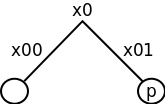
\includegraphics[scale=0.4]{Figures/Protocol/conPeer_route1equiv.png}
        \caption{Peer p στο μονοπάτι route1 και peer στο συζυγές μονοπάτι}
        \label{fig:Route1Case1a}
    \end{subfigure}
    \quad
    \begin{subfigure}[b]{0.3\textwidth}
        \centering
        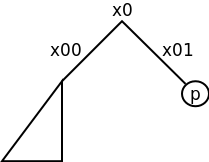
\includegraphics[scale=0.4]{Figures/Protocol/conSubtree_route1equiv.png}
        \caption{Peer p στο μονοπάτι route1 και υπόδεντρο στο συζυγές μονοπάτι}
        \label{fig:Route1Case1b}
    \end{subfigure}
    \quad
    \begin{subfigure}[b]{0.3\textwidth}
        \centering
        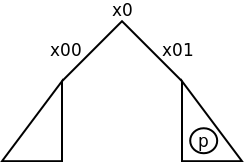
\includegraphics[scale=0.4]{Figures/Protocol/conSubtree_route1subtree.png}
        \caption{Το μονοπάτι route1 είναι πρόθεμα σε υπόδεντρο που περιέχει τον peer p}
        \label{fig:Route1Case2}
    \end{subfigure}
    \caption{Περιπτώσεις κατά την επιλογή της κατεύθυνσης \textit{route1 $\equiv$ 'x01'}}
    \label{fig:Route1}
\end{figure}

Αρχικά ελέγχουμε το μονοπάτι του peer που εκτελεί τον αλγόριθμο με τη πρώτη 
διαδρομή \textit{route1}. Στη γραμμή \ref{code:CheckRoute1} αποφασίζεται αν 
ο peer έχει πρόθεμα το \textit{route1}. Αν η απάντηση είναι αληθής τότε 
διακρίνουμε τρεις περιπτώσεις που πρέπει να ελέγξουμε. Οι περιπτώσεις αυτές 
είναι που βρίσκεται ο peer που εκτελεί τον αλγόριθμο και τι συμβαίνει στο 
συζυγές μονοπάτι του \textit{route1}. Ένας πρώτος διαχωρισμός είναι αν 
το μονοπάτι του peer είναι όμοιο με το \textit{route1} ή όχι. Ο έλεγχος 
φαίνεται στη γραμμή \ref{code:Route1Equiv}. 

Για την περίπτωση της ομοιότητας για να αποφανθούμε τι τελικά θα ακολουθήσουμε 
πρέπει να εξετάσουμε το συζυγές μονοπάτι του \textit{route1}. Εδώ έχουμε δυο 
περιπτώσεις, η πρώτη είναι το συζυγές να αντιστοιχεί σε μόνο ένα peer και 
εξετάζεται στη γραμμή \ref{code:Route1EquivConPeer}. Η κατάσταση αυτή φαίνεται 
ξεκάθαρα στο σχήμα\ref{fig:Route1Case1a}. Ο αλγόριθμος τερματίζει και 
επιστρέφεται ο peer \textit{p} που τον εκτέλεσε. Η διάσχιση οδήγησε σε δυο 
φύλλα του δέντρου του P-Grid και οι δυο peer που αντιστοιχούν σε αυτά μπορούν 
να λύσουν την αποτυχία. Αντίθετα στη γραμμή \ref{code:Route1EquivConSubtree} 
καταλήγουμε αν το συζυγές μονοπάτι αντιστοιχεί σε ένα υπόδεντρο που περιέχει 
άνω του ενός peer. Η κατάσταση απεικονίζεται στο σχήμα \ref{fig:Route1Case1b}, 
δεν έχουμε φτάσει σε φύλλα. Όμως, οι δυο peer που θα δώσουν την λύση βρίσκονται 
στο υπόδεντρο αυτό. Συνεπώς, ο αλγόριθμος τερματίζει επιστρέφοντας έναν peer 
που βρίσκεται στον πίνακα δρομολόγησης του \textit{p}. Αυτός ανήκει στο συζυγές 
υπόδεντρο του \textit{route1}, έχοντας δηλαδή πρόθεμα το \textit{route2}. 
Στο σχήμα \ref{fig:Route1Case1b} είναι στο 'x00'. 

Η τελική περίπτωση που έχουμε για την διαδρομή \textit{route1} 
είναι στη γραμμή \ref{code:Route1Subtrees} όπου η διαδρομή είναι πρόθεμα ενός 
υποδέντρου. Στο συζυγές υπόδεντρο δε μας ενδιαφέρει τι γίνεται. 
Ανεξάρτητα του αριθμού των peer που βρίσκονται σε αυτό, οι peer που θα δώσουν 
την λύση βρίσκονται στο υπόδεντρο με πρόθεμα \textit{route1}. 
Η επιλογή της διαδρομής στην περίπτωση αυτή γίνεται κατά σύμβαση. Ο αλγόριθμος 
συνεχίζει αναδρομικά εξειδικεύοντας σε αυτό το υπόδεντρο μέχρι να φτάσει σε 
διαδρομή που αντιστοιχεί σε έναν peer ακριβώς. 

\begin{figure}[ht]
    \centering
    \begin{subfigure}[b]{0.3\textwidth}
        \centering
        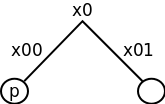
\includegraphics[scale=0.4]{Figures/Protocol/route2equiv_conPeer.png}
        \caption{Peer p στο μονοπάτι route2 και peer στο συζυγές μονοπάτι}
        \label{fig:Route2Case1a}
    \end{subfigure}
    \quad
    \begin{subfigure}[b]{0.3\textwidth}
        \centering
        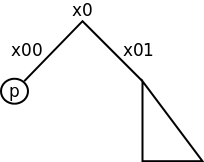
\includegraphics[scale=0.4]{Figures/Protocol/route2equiv_conSubtree.png}
        \caption{Peer p στο μονοπάτι route2 και υπόδεντρο στο συζυγές μονοπάτι}
        \label{fig:Route2Case1b}
    \end{subfigure}
    \quad
    \begin{subfigure}[b]{0.3\textwidth}
        \centering
        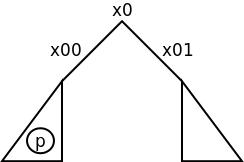
\includegraphics[scale=0.4]{Figures/Protocol/route2subtree_conSubtree.png}
        \caption{Το μονοπάτι route2 είναι πρόθεμα σε υπόδεντρο που περιέχει τον peer p}
        \label{fig:Route2Case2}
    \end{subfigure}
    \caption{Περιπτώσεις κατά την επιλογή της κατεύθυνσης \textit{route2 $\equiv$ 'x00'}}
    \label{fig:Route2}
\end{figure}

Αν ο peer \textit{p} δεν έχει πρόθεμα το μονοπάτι \textit{route1} τότε 
βρίσκεται στο \textit{route2}. Ο έλεγχος φαίνεται στην γραμμή 
\ref{code:CheckRoute2}. Αντίστοιχα και εδώ έχουμε παρόμοιες περιπτώσεις απλά 
αλλάζει η θέση του peer \textit{p}. 

Συγκεκριμένα, στην γραμμή \ref{code:Route2Equiv} κρίνεται αν ο π \textit{p} 
έχει μονοπάτι όμοιο με το \textit{route2}. Η περίπτωση που απεικονίζεται στο 
σχήμα \ref{fig:Route2Case1a}, όπου \textit{route2} είναι ίσο με 'χ00', 
αντιστοιχεί στην επαλήθευση του ελέγχου στην γραμμή 
\ref{code:Route1EquivConPeer}. Ο αλγόριθμος έχει οδηγηθεί σε φύλλα και άρα 
έχουν βρεθεί οι peer που θα λύσουν το πρόβλημα. Επιστρέφεται επομένως ο peer 
\textit{p}. Αντίθετα, αν έχουμε συζυγές υπόδεντρο με πρόθεμα \textit{route1}, 
τότε το ακολουθούμε επιστρέφοντας έναν peer που ανήκει σε αυτό. Στο σχήμα 
\ref{fig:Route2Case1b} φαίνεται η περίπτωση αυτή.

Τέλος, στην γραμμή \ref{code:Route2Subtrees} είναι η περίπτωση όπου η 
διαδρομή \textit{route2} είναι πρόθεμα στο υπόδεντρο που ανήκει ο \textit{p}. 
Ο αλγόριθμος συνεχίζει αναδρομικά προς αυτή την διαδρομή ώστε να εξειδικευτεί 
περισσότερο και να καταλήξουμε σε διαδρομή που αντιστοιχεί σε peer.

\begin{algorithm}
\caption{Αλγόριθμος FindContinuation}
\label{algo:Continuation}
\begin{algorithmic}[1]
    \Procedure{p.FindContinuation}{pathTrace}
        \If{path(p) $\equiv$ pathTrace} \label{code:Check1}
            \State \Return p
        \EndIf
        \If{p.isPrefixOf(pathTrace) $\cup$ (path(p).length() $\leq$ pathTrace.length())} \label{code:Check2}
            \State \Return p.closestLevelTo(pathTrace)
        \EndIf
        \State route1 $\gets$ pathTrace + $\neg$pathTrace.lastBit() \label{code:PathRoute1}
        \State route2 $\gets$ pathTrace + pathTrace.lastBit() \label{code:PathRoute2}
        \If{p.hasPrefix(route1)} \label{code:CheckRoute1}
            \If{path(p) $\equiv$ route1} \label{code:Route1Equiv}
                \If{p has conjugate peer and not a subtree} \label{code:Route1EquivConPeer}
                    \State \Return p
                \Else \label{code:Route1EquivConSubtree}
                    \State \Return p.closestLevelTo(route2)
                \EndIf
            \Else \label{code:Route1Subtrees}
                \State \Return p.FindContinuation(route1)
            \EndIf
        \ElsIf{p.hasPrefix(route2)} \label{code:CheckRoute2}
            \If{path(p) $\equiv$ route2} \label{code:Route2Equiv}
                \If{p has conjugate peer and not a subtree} \label{code:Route2EquivConPeer}
                    \State \Return p
                \Else \label{code:Route2EquivConSubtree}
                    \State \Return p.closestLevelTo(route1)
                \EndIf
            \Else \label{code:Route2Subtrees}
                \State \Return p.FindContinuation(route2)
            \EndIf
        \EndIf

    \EndProcedure
\end{algorithmic}
\end{algorithm}

\subsubsection{Αλγόριθμος Replace}
Ο αλγόριθμος επιδιόρθωσης θα καταλήξει σε έναν peer. Αυτός μαζί με τον 
συζυγή του πρόκειται να δώσουν την λύση στην αποτυχία. Ο αλγόριθμος 
\ref{algo:Replace} (Replace) δείχνει τον τρόπο. Συγκεκριμένα, ο ένας από 
τους δυο peer θα λάβει το μονοπάτι που αντιστοιχεί στην αποτυχία. Ο δεύτερος 
θα μειώσει το μονοπάτι του κατά ένα, δηλαδή γενικεύεται. Υπενθυμίζουμε πως 
ως αποτυχία θεωρείται είτε ένας peer, είτε ένα το σύνολο των peer ενός 
υποδέντρου. Από σύμβαση, ο peer του οποίου το μονοπάτι καταλήγει σε '1', 
είναι αυτός που θα αντικαταστήσει. Τέλος, ανανεώνουν τον πίνακα 
δρομολόγησης. Στην απλή περίπτωση που η αποτυχία 
είναι ο συζυγής peer, τότε απλά μειώνεται το μονοπάτι κατά ένα. 
Ο αλγόριθμος \ref{algo:Replace} εκτελείται ταυτόχρονα από τους δύο peer 
που είναι υπεύθυνοι για λύση. Όταν τερματίσει και από τους δυο τότε, οι 
δυο peer έχουν διορθώσει το πρόβλημα. Το επόμενο βήμα είναι η αναμετάδοση 
της λύσης μέσα στο δίκτυο.

\begin{algorithm}
\caption{Αλγόριθμος Replace}
\label{algo:Replace}
\begin{algorithmic}[1]
    \Procedure{p.Replace}{failed}
        \If{failed.isConjugateTo(p)}
            \State path(p).reduceBy(1)
        \Else
            \If{path(p).endsWith('1')}
	            \State path(p) $\gets$ path(failed)
            \Else
                \State path(p).reduceBy(1)
            \EndIf
        \EndIf
        \State p.refreshRoutingTable()
    \EndProcedure
\end{algorithmic}
\end{algorithm}

\subsubsection{Αλγόριθμος Broadcast}
Ο αλγόριθμος \ref{algo:Broadcast} (Broadcast) είναι υπεύθυνος για την διάδοση 
της λύσης στο δίκτυο. Ο peer στον οποίο θα καταλήξει ο αλγόριθμος επιδιόρθωσης % ref
για να διορθώσει το πρόβλημα είναι αυτός που θα καλέσει την μέθοδο 
\textit{InitBroadcast}. Τα ορίσματα που απαιτούνται είναι 
\begin{inparaenum}[\itshape (a)\upshape]
\item το μονοπάτι που αντιστοιχεί στην αποτυχία είτε αυτή είναι μεμονωμένος
peer είτε ολόκληρο υπόδεντρο,
\item μια λίστα με όλους τους peer που εξαιτίας της επίλυσης άλλαξαν την 
κατάστασή τους και
\item μια λίστα με όλους τους αποτυχημένους peer που έχουν πρόθεμα το 
προαναφερθέν μονοπάτι.
\end{inparaenum}
Η λίστα με τους ανανεωμένους peer περιέχει τον peer που εκκινεί τον 
αλγόριθμο και τον συζυγή του. Σε αυτούς κατέληξε ο αλγόριθμος επιδιόρθωσης 
και συνεπώς αυτοί θα αλλάξουν το μονοπάτι τους ώστε να λύσουν την αποτυχία. 
Αρχικά ανανεώνεται ο πίνακας δρομολόγησης αφαιρώντας όλους τους peer που 
έχουν αποτύχει. Στη συνέχεια για κάθε επίπεδο που έχει αποθηκευμένο στον 
πίνακα δρομολόγησης του, επιλέγει τυχαία έναν peer από αυτό και του προωθεί 
την λύση. 

Στη συνέχεια, οι υπόλοιποι peer εκτελούνε την μέθοδο \textit{Broadcast}. 
Η μέθοδος αυτή έχει τα ίδια ορίσματα με την \textit{InitBroadcast} και 
επιπλέον ένα, το \textit{subtree}. Αυτό υποδηλώνει στον peer πιο είναι το 
υπόδεντρο για το οποίο είναι υπεύθυνος να προωθήσει την λύση. Όπως μπορούμε 
να δούμε από τον ψευδοκώδικα, κάθε peer είναι υπεύθυνος για το υπόδεντρο στο 
οποίο ανήκει. Ο λόγος για τον οποίο γίνεται αυτό είναι ο περιορισμός του 
αριθμού των μηνυμάτων που πρέπει να στείλουμε. Σε αντίθετη περίπτωση πολλοί 
peer θα δεχόντουσαν πολλαπλά μηνύματα για την ίδια λύση. Ο peer αφαιρεί από 
τον πίνακα δρομολόγησης του τους αποτυχημένους peer. Αν έχει αναφορές σε 
αυτούς που έχουν αλλάξει κατάσταση, τις ενημερώνει, αλλιώς 
τους προσθέτει στον πίνακα. Καταλήγει προωθώντας την λύση επιλέγοντας τυχαία 
έναν peer για κάθε επίπεδο του πίνακα που έχει πρόθεμα το μονοπάτι του 
υποδέντρου για το οποίο είναι υπεύθυνος. Ένας peer δεν εκτελεί τον αλγόριθμο 
όταν το μονοπάτι ευθύνης είναι όμοιο με το μονοπάτι του. Αυτό σημαίνει πως 
δεν υπάρχουν peer περισσότερο εξειδικευμένοι από αυτόν.

\begin{algorithm}
\caption{Αλγόριθμος Broadcast}
\label{algo:Broadcast}
\begin{algorithmic}[1]
    \Procedure{p.InitBroadcast}{failedPath, updatedHosts, failedHosts}
        \State p.updateRoutingTable(failedHosts)
        \ForAll{level in RoutingTable}
            \State p' $\gets$ level.selectRandomHost()
            \State subtree $\gets$ path(level)
            \State p'.broadcast(failedPath, updatedHosts, failedHosts, subtree)
        \EndFor
    \EndProcedure
    \Statex
    \Procedure{p.Broadcast}{failedPath, updatedHosts, failedHosts, subtree}
        \State p.updateRoutingTable(failedHosts, updatedHosts)
        \If{path(p) $\equiv$ subtree}
            \State \Return
        \EndIf
        \ForAll{level in RoutingTable.levelsIn(subtree)}
            \State p' $\gets$ level.selectRandomHost()
            \State subtree $\gets$ path(level)
            \State p'.broadcast(failedPath, updatedHosts, failedHosts, subtree)
        \EndFor
    \EndProcedure
\end{algorithmic}
\end{algorithm}

\subsection{Ανάλυση Πρωτοκόλλου}

Το πρωτόκολλο μπορεί να αντιμετωπίσει είτε μεμονωμένες αποτυχίες peer είτε 
την αποτυχία ενός πλήρους υποδέντρου του δικτύου. Πριν εξηγηθούν τα βήματα 
που εκτελούνται σε κάθε περίπτωση, θα εξηγηθεί μια δομή που χρησιμοποιείται 
κατά την επίλυση προβλημάτων.

Χρησιμοποιείται ένας πίνακας καταχώρησης (registry) των αποτυχιών που 
προκύπτουν κατά τη διάρκεια ζωής του συστήματος. Οι καταχωρήσεις αυτές 
παραμένουν μέχρι τη στιγμή που επιλυθούν τα προβλήματα. Προϋπόθεση είναι η 
λήψη μηνύματος που περιέχει την λύση μέσω του αλγορίθμου Broadcast.

Όταν ανακαλυφθεί ένας peer που έχει αποτύχει τότε το σύστημα προσπαθεί να 
τον διορθώσει βρίσκοντας το σωστό ζευγάρι για την αντικατάσταση του. Συνεπώς, 
το πρωτόκολλο ξεκινά πάντα με επίλυση αποτυχίας μεμονωμένου peer. Είναι αρκετά 
πιθανό η αποτυχία να ανακαλυφθεί και να εκκινηθεί το πρωτόκολλο ταυτόχρονα από 
πολλούς peer. Επομένως, το πρώτο που γίνεται είναι ο έλεγχος της registry και 
η ανανέωση του πίνακα δρομολόγησης όπου αφαιρείται οποιαδήποτε αναφορά προς 
τον προβληματικό peer. Αν μέσα στην registry βρεθεί το ID του αποτυχημένου peer 
τότε σημαίνει πως το πρωτόκολλο έχει τρέξει και αναμένει για την λύση.

\subsubsection{Επίλυση αποτυχίας μεμονομένου peer}

Αν στην registry δεν βρεθεί ο αποτυχημένος peer τότε εκτελείται εκείνο το 
κομμάτι του πρωτοκόλλου που επιλύει αποτυχία ενός μεμονωμένου peer.

Αρχικά εκτελείται ο αλγόριθμος FindContinuation (\ref{algo:Continuation}). 
Αυτός θα επιλέξει έναν peer για την συνέχιση του πρωτοκόλλου όπως αναλύθηκε 
προηγουμένως. Αν ο peer είναι ένας από τον πίνακα δρομολόγησης και δεν είναι 
ο τοπικός, αυτός που εκτελεί τον αλγόριθμο δηλαδή, τότε σημαίνει πως ακόμα δεν 
έχουμε φτάσει σε φύλλα. Μπορούμε να θυμηθούμε τα σχήματα 
\ref{fig:Route1Case1b}, \ref{fig:Route2Case1b}, \ref{fig:Route1Case2} 
και \ref{fig:Route2Case2} για να καταλάβουμε γιατί.

Αν αυτός ο peer είναι ο τοπικός τότε σημαίνει πως αυτός είναι σε θέση να επιλύσει την αποτυχία. 
Για υπενθύμιση μπορούμε να δούμε τις εικόνες \ref{fig:Route1Case1a} και 
\ref{fig:Route2Case1a} για να καταλάβουμε τον λόγο. Ο αλγόριθμος έχει φτάσει 
σε φύλλα. Για την συνέχεια έχουμε δυο περιπτώσεις που έχουν να κάνουν με τον 
συζυγή του τοπικού. Ο συζυγής του μπορεί είτε να είναι ο αποτυχημένος peer 
που προσπαθεί το δίκτυο να επιλύσει. Τότε μέσω της εκτέλεσης του αλγορίθμου 
Replace (\ref{algo:Replace}), ο τοπικός ελαττώνει το μονοπάτι του κατά ένα. Στην 
περίπτωση που ο συζυγής είναι διαθέσιμος τότε ο τοπικός του στέλνει αίτηση 
εκτέλεσης του αλγορίθμου Replace για τον αποτυχημένο peer. Όπως αναλύθηκε 
παραπάνω, ο ένας peer θα πάρει το μονοπάτι του αποτυχημένου και ο άλλος θα 
ελαττώσει κατά ένα το μονοπάτι του.

Το τελικό βήμα του πρωτοκόλλου εκτελείται από τον peer που θα εκτελέσει τον 
αλγόριθμο Replace. Εκτελεί τον αλγόριθμο Broadcast (\ref{algo:Broadcast}) 
ώστε η λύση να διαδοθεί σε όλο το δίκτυο. Αφού ανανεωθεί ο 
πίνακας δρομολόγησης ενός peer που έχει λάβει την λύση, μόνο τότε διαγράφει 
την καταχώρηση του αποτυχημένου peer από την registry. Αυτό αφορά εκείνους 
τους peer που συμμετείχαν ενεργά στην εκτέλεση του πρωτοκόλλου. Όσοι δεν 
πήραν μέρος πιθανώς να μη γνωρίζουν για την αποτυχία. Δεν έχουμε πρόβλημα 
όμως αφού ο πίνακας δρομολόγησης τους ανανεώνεται με τους νέους peer και 
επομένως μαθαίνουν την καινούρια κατάσταση του δικτύου.

\subsubsection{Επίλυση αποτυχίας ενός πλήρους υποδέντρου}

